\documentclass[11pt]{article}

\usepackage[margin=1in]{geometry}
\usepackage[T1]{fontenc}
\usepackage{lmodern}
\usepackage{microtype}
\usepackage{booktabs}
\usepackage{array}
\usepackage{xcolor}
\usepackage{hyperref}
\usepackage[american]{circuitikz}
\usetikzlibrary{arrows.meta,calc,decorations.pathreplacing,positioning}

\hypersetup{
  colorlinks=true,
  linkcolor=blue!50!black,
  urlcolor=blue!50!black
}

\title{Toyota OBD1 Bench Simulator and Arduino Receiver}
\author{Raspberry Pi GPIO21 to Arduino D7}
\date{2026-06-07}

\begin{document}
\maketitle

\section{Goal}

The task was to build a Raspberry Pi based Toyota OBD1 signal simulator.
The Arduino acts as the receiver, so the Python simulator is the reverse of
the Arduino receive logic.  The bench wire is:
\[
  \text{Raspberry Pi BCM GPIO21} \rightarrow \text{Arduino D7}.
\]
Only the CH340 USB serial path is used for Arduino status.  The display,
SD-card, EEPROM, injector, and button peripherals from the reference project
are intentionally removed.

\section{Reference}

The protocol constants and receive state machine were taken from the
\texttt{hyperion11/toyota-obd-1} project:
\[
  \url{https://github.com/hyperion11/toyota-obd-1}.
\]
The relevant receiver behavior is in \texttt{OBD.ino}: long HIGH preamble,
8 ms bit cells, four ID bits, and data bytes with one LOW start bit, eight
LSB-first data bits, and two HIGH stop bits.

\section{Bench Circuit}

The real Toyota diagnostic VF1 line can be a vehicle-level signal and must
not be connected directly to a Raspberry Pi or Arduino input.  This bench
test does not use the vehicle line; it uses the Raspberry Pi 3.3 V GPIO as
the simulated source.  Grounds must be common.

\begin{figure}[h]
\centering
\begin{circuitikz}[american, thick]
  \node[draw, rounded corners=2pt, minimum width=3.3cm, minimum height=2.2cm]
    (pi) {Raspberry Pi};
  \node[draw, rounded corners=2pt, minimum width=3.6cm, minimum height=2.2cm,
    right=4.6cm of pi] (uno) {Arduino Uno};

  \coordinate (pigpio) at ($(pi.east)+(0,0.45)$);
  \coordinate (unopin) at ($(uno.west)+(0,0.45)$);
  \coordinate (pignd) at ($(pi.east)+(0,-0.55)$);
  \coordinate (unognd) at ($(uno.west)+(0,-0.55)$);

  \draw (pigpio) node[left=2pt] {\small GPIO21}
    to[R,l=$1\,\mathrm{k\Omega}$] (unopin)
    node[right=2pt] {\small D7};

  \draw (pignd) node[left=2pt] {\small GND}
    -- (unognd) node[right=2pt] {\small GND};

  \draw ($(pignd)!0.5!(unognd)$) -- ++(0,-0.5) node[ground] {};
  \node[above=0.2cm of pigpio, align=center, font=\small]
    {3.3 V logic source\\Pi drives, Arduino receives};
\end{circuitikz}
\caption{Bench wiring for the simulator.  The resistor is optional for this
one-way bench signal, but it limits fault current during development.}
\end{figure}

\section{Signal Format}

The receiver watches signal edges and uses elapsed time to count 8 ms bit
cells.  A packet begins when the line has been HIGH longer than 15 bit cells
and then falls LOW.  The final packet is committed on the next falling edge
after the HIGH stop/trailer period, matching the continuous Toyota stream.

\begin{table}[h]
\centering
\begin{tabular}{@{}lll@{}}
\toprule
Field & Wire level & Duration \\
\midrule
Preamble/trailer & HIGH & $> 15 \times 8$ ms; bench uses 160 ms \\
Packet start edge & HIGH to LOW & edge only \\
ID & normal bit level & 4 bits, LSB first \\
Byte start & LOW & 1 bit \\
Byte data & normal bit level & 8 bits, LSB first \\
Byte stop & HIGH & 2 bits \\
\bottomrule
\end{tabular}
\end{table}

\begin{figure}[h]
\centering
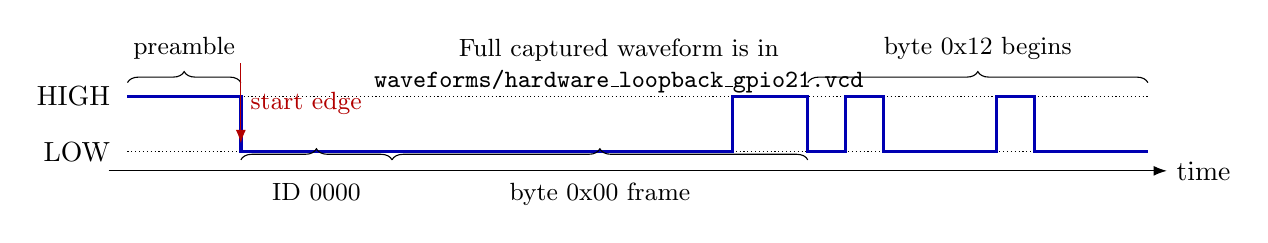
\begin{tikzpicture}[x=0.48cm,y=0.7cm,>=Latex]
  \draw[->] (-0.5,-0.35) -- (27.5,-0.35) node[right] {time};
  \draw (-0.2,0) node[left] {LOW};
  \draw (-0.2,1) node[left] {HIGH};
  \draw[densely dotted] (0,0) -- (27,0);
  \draw[densely dotted] (0,1) -- (27,1);

  % Preamble, packet start, ID 0x0, byte 0x00, byte 0x12, with omissions.
  \draw[very thick, blue!70!black]
    (0,1) -- (3,1)
    -- (3,0) -- (7,0)
    -- (7,0) -- (16,0)
    -- (16,1) -- (18,1)
    -- (18,0) -- (19,0)
    -- (19,1) -- (20,1)
    -- (20,0) -- (23,0)
    -- (23,1) -- (24,1)
    -- (24,0) -- (27,0);

  \draw[decorate, decoration={brace, amplitude=4pt}]
    (0,1.25) -- (3,1.25) node[midway,above=5pt] {\small preamble};
  \draw[decorate, decoration={brace, amplitude=4pt}]
    (3,-0.15) -- (7,-0.15) node[midway,below=5pt] {\small ID 0000};
  \draw[decorate, decoration={brace, amplitude=4pt}]
    (7,-0.15) -- (18,-0.15) node[midway,below=5pt] {\small byte 0x00 frame};
  \draw[decorate, decoration={brace, amplitude=4pt}]
    (18,1.25) -- (27,1.25) node[midway,above=5pt] {\small byte 0x12 begins};

  \draw[red!70!black, -Latex] (3,1.6) -- (3,0.15)
    node[midway,right] {\small start edge};
  \node[font=\small, align=center] at (13,1.55)
    {Full captured waveform is in\\\texttt{waveforms/hardware\_loopback\_gpio21.vcd}};
\end{tikzpicture}
\caption{Simplified wire waveform.  Consecutive equal bits are held as a
single longer level; the Arduino reconstructs bit count from edge spacing.}
\end{figure}

\section{Implementation}

\begin{itemize}
  \item Arduino receiver:
    \texttt{arduino\_code/ToyotaOBD1Receiver/ToyotaOBD1Receiver.ino}
  \item Python simulator:
    \texttt{python\_code\_aka\_obd1\_simulator/toyota\_obd1\_sim.py}
  \item Hardware loopback test:
    \texttt{python\_code\_aka\_obd1\_simulator/hardware\_loopback\_test.py}
  \item GTKWave files:
    \texttt{waveforms/hardware\_loopback\_gpio21.vcd} and
    \texttt{waveforms/hardware\_loopback\_gpio21.gtkw}
\end{itemize}

The Arduino uses the ATmega328P pin-change interrupt for D7 because D7 is not
one of the Uno external interrupt pins.  The packet decode state machine is
otherwise kept equivalent to the reference edge-duration logic.

\section{Build, Upload, and Test}

The Arduino board was visible as \texttt{/dev/ttyUSB0} with the CH340 connected
to the ATmega.  The sketch was compiled with:

\begin{verbatim}
arduino-cli compile --fqbn arduino:avr:uno \
  --build-path /tmp/arduino-build-toyota-obd1 \
  arduino_code/ToyotaOBD1Receiver
\end{verbatim}

Compile result:

\begin{verbatim}
Sketch uses 5654 bytes (17%) of program storage space.
Global variables use 261 bytes (12%) of dynamic memory.
\end{verbatim}

The compiled sketch was uploaded with:

\begin{verbatim}
arduino-cli upload -p /dev/ttyUSB0 --fqbn arduino:avr:uno \
  --input-dir /tmp/arduino-build-toyota-obd1
\end{verbatim}

The hardware loopback test command was:

\begin{verbatim}
python3 python_code_aka_obd1_simulator/hardware_loopback_test.py \
  --port /dev/ttyUSB0 --gpio 21 --count 3
\end{verbatim}

Result:

\begin{verbatim}
READY toyota_obd1_receiver input=D7 serial=115200 bit_cell_ms=8
PACKET id=0x0 bytes=15 raw=00 12 67 5F 2C 01 E4 00 3C 80 00 20 82 08 30
PACKET id=0x0 bytes=15 raw=00 12 67 5F 2C 01 E4 00 3C 80 00 20 82 08 30
PACKET id=0x0 bytes=15 raw=00 12 67 5F 2C 01 E4 00 3C 80 00 20 82 08 30
PASS packets_seen=3 expected_raw=00 12 67 5F 2C 01 E4 00 3C 80 00 20 82 08 30
\end{verbatim}

The decoded values from the Arduino were:
\[
\mathrm{INJ}=2.25\ \mathrm{ms},\quad
\mathrm{IGN}=18.4^\circ,\quad
\mathrm{RPM}=1100,\quad
\mathrm{ECT}=80.0^\circ\mathrm{C},\quad
\mathrm{SPD}=60\ \mathrm{km/h}.
\]

\section{GTKWave}

The simulator and hardware test both write VCD and GTKWave save files.  On a
machine with GTKWave installed, open the captured hardware waveform with:

\begin{verbatim}
gtkwave waveforms/hardware_loopback_gpio21.gtkw
\end{verbatim}

In this session, \texttt{gtkwave} and \texttt{pdflatex} were not installed, and
\texttt{sudo apt-get} could not run because a password was required.  The
LaTeX source and GTKWave input files are complete and ready to build once those
tools are installed.

\end{document}
